\documentclass[12pt]{beamer}
%\includeonlyframes{current}

\mode<presentation>{\usetheme{Warsaw}}
\setbeamertemplate{footline}[frame number]
\usepackage[english]{babel}
\usepackage{times}
\usepackage{url}
\usepackage{graphicx}
\usepackage{listings}
\usepackage{hhline}
\usepackage{array}
\usepackage{colortbl}
\usepackage{changepage}
\lstloadlanguages{Python}
\lstset{language=Python}
\lstset{%
	basicstyle=\ttfamily\bfseries,
	keywordstyle=\color{blue}, emph={self}, emphstyle={\color{blue}},
	identifierstyle=,
	commentstyle=\color{gray},
	stringstyle=\color{green!50!black},
	showstringspaces=false,
	emph={[2]__init__,__str__}, emphstyle={[2]\color{purple}},
}
\newcommand{\key}[1]{{\color{blue}#1}}
\newcommand{\cmnt}[1]{{\color{gray}#1}}
\newcommand{\str}[1]{{\color{green!50!black}#1}}
\newcommand{\defn}[1]{{\color{purple}#1}}
\newcommand{\SC}[1]{\mbox{\sc#1}}
\newcommand{\EM}[1]{\mbox{\em#1}}
\newcommand{\EMSCR}[1]{\mbox{\em\scriptsize#1}}
\newcommand{\tab}{\hspace{1em}}

\newlength{\cellwidth}
\setlength{\cellwidth}{.5in}
\newcommand{\cell}[1]{\parbox[c][\cellwidth]{\cellwidth}{#1}}
\newcommand{\emptycell}{\cell{\ }}
\newcommand{\wumpcell}[2]{\cell{%
	\centering
	\vspace{.1\cellwidth}
	\parbox[c][.2\cellwidth]{.9\cellwidth}{\scriptsize #1} \\
	\vspace{.1\cellwidth}
	\parbox[c][.5\cellwidth]{.9\cellwidth}{\centering #2}}}
\newcommand{\tinywumpcell}[2]{\cellwidth=.25in\cell{%
	\centering
	\vspace{.1\cellwidth}
	\parbox[c][.45\cellwidth]{.95\cellwidth}{\tiny #1} \\[-.3\cellwidth]
	\parbox[c][.45\cellwidth]{.95\cellwidth}{\tiny\centering #2}}}
\newcommand{\tinywumpusworld}[6]{
	\begin{tabular}{@{}|@{}l@{}|@{}l@{}|@{}l@{}|@{}l@{}|@{}}
		\hhline{-~~}
		\tinywumpcell{1,3}{#1} &
		\multicolumn{2}{c}{} \\
		\hhline{--~}
		\tinywumpcell{1,2}{#2} &
		\tinywumpcell{2,2}{#3} &
		\multicolumn{1}{c}{} \\
		\hline
		\tinywumpcell{1,1}{#4} &
		\tinywumpcell{2,1}{#5} &
		\tinywumpcell{3,1}{#6} \\
		\hline
	\end{tabular}
}


\title{Uncertainty}
\subtitle{Introduction to Artificial Intelligence}
\author{Steven Bethard}
\institute{
  Department of Computer Science\\
  University of Colorado
}
\date{CSCI 3202}


\AtBeginSection[]{
\begin{frame}<beamer>{Outline}
	\tableofcontents[currentsection]
\end{frame}
}

\begin{document}

\begin{frame}
	\titlepage
\end{frame}

\section{Probability Theory}
\begin{frame}{Motivation}
	\begin{block}{Goal}
		Look out window - is it warm?
	\end{block}
	\pause
	\begin{block}{Rules}
		$
		\begin{array}{l}
			\forall d\ \EM{Sunny}(d) \Rightarrow \EM{Warm}(d) \\
			\pause \mbox{Wrong; it can be sunny but cold} \\
			\pause \forall d\ \EM{Warm}(d) \Rightarrow \EM{Sunny}(d) \\
			\pause\mbox{Wrong; it can be warm and cloudy} \\
		\end{array}
		$
	\end{block}
	\pause
	\begin{block}{Problem}
		Can't capture that sunny days are usually warm
	\end{block}
\end{frame}


\subsection{Probability Basics}
\begin{frame}{Probability Theory}
	\begin{block}{Key Idea}
		Measure degrees of belief in propositions
	\end{block}
	\bigskip
	\begin{tabular}{@{}l@{\hspace{.5em}}l@{}}
		\pause
		\key{Random Variable} & An interesting part of the world \\
		                      & e.g. $\EM{Sky}$ or $\EM{Temp}$ \\[.5em]
		\pause
		\key{Domain}          & Possible values of a random variable \\
		                      & e.g. $\EM{domain}(\EM{Temp})=\langle\EM{warm}, \EM{cold}, \ldots\rangle$ \\[.5em]
		\pause
		\key{Proposition}     & A statement, like propositional logic \\
		                      & e.g. $\EM{Sky}\!=\!\EM{sunny} \land \EM{Temp}\!=\!\EM{warm}$ \\[.5em]
		\pause
		\key{Probability}     & The degree of belief in a proposition \\
		                      & e.g. $P(\EM{Temp}\!=\!\EM{warm}) = 0.7$
	\end{tabular}
\end{frame}
\begin{frame}{Aside: Fuzzy Logic}
	\begin{block}{Probability Theory}
		\begin{itemize}
			\item Propositions are believed to a certain degree
			\item Belief values range from [0, 1]
		\end{itemize}
	\end{block}
	\pause
	\begin{block}{Fuzzy Logic}
		\begin{itemize}
			\item Propositions are \EM{true} to a certain degree
			\item \EM{Truth} values range from [0, 1]
		\end{itemize}
		\pause
		For example:
		\begin{itemize}
			\item $T(\EM{Tall}(\EM{Steve})) = 0.5$
			\item $T(\EM{Fat}(\EM{Steve})) = 0.1$
		\end{itemize}
		\pause
		Better for describing indefinite classes than for reasoning
	\end{block}
\end{frame}
\begin{frame}{Probability Rules}
	\begin{block}{Range of Probabilities}
		$0 \leq P(a) \leq 1$
	\end{block}
	\pause
	\begin{block}{Propositions Known to be True or False}
		$
		\begin{array}{lll}
			P(\EM{true})  & = & 1 \\
			P(\EM{false}) & = & 0 \\
		\end{array}
		$
	\end{block}
	\pause
	\begin{block}{Probability of Disjunctions}
		\begin{tabular}{lc}
			$
			\begin{array}{lc}
				\lefteqn{P(a \lor b) = \mbox{}} \\[.5em]
				& P(a) + P(b) - P(a \land b)
			\end{array}
			$
			&
			\pause
			\parbox{1.25in}{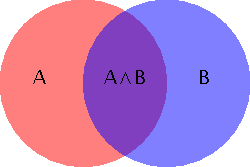
\includegraphics[width=1.25in]{venn}}
		\end{tabular}
	\end{block}
\end{frame}
\begin{frame}{Random Variables}
	\begin{block}{Boolean Random Variables}
		Have the domain $\langle \EM{true}, \EM{false} \rangle$, e.g.
		\begin{itemize}
			\item \EM{IsSunny}
		\end{itemize}
	\end{block}
	\pause
	\begin{block}{Discrete Random Variables}
		Have a countable domain, e.g.
		\begin{itemize}
			\item $\EM{domain}(\EM{Sky}) =
			       \langle \EM{sunny}, \EM{cloudy}, \ldots \rangle$
			\item $\EM{domain}(\EM{DieRoll}) =
			       \langle 1, 2, 3, 4, 5, 6 \rangle$
		\end{itemize}
	\end{block}
	\pause
	\begin{block}{Continuous Random Variables}
		Have a real-valued domain, e.g.
		\begin{itemize}
			\item $\EM{domain}(\EM{Temperature}) =
			       \langle \ldots, -40^{\circ}, \ldots, 98.6^{\circ}, \ldots \rangle$
		\end{itemize}
	\end{block}
\end{frame}


\subsection{Prior, Joint and Conditional Probabilities}
\begin{frame}{Prior Probability}
	\begin{block}{Definition}
		\begin{tabular}{lm{3.5in}}
			\large $P(a)$
			&
			The \alert{unconditional} or \alert{prior probability} of a proposition $a$ is the degree of belief in that proposition \emph{given no other information}
		\end{tabular}
	\end{block}
	\pause
	\begin{block}{Examples}
		$
		\begin{array}{lll}
			P(\EM{DieRoll} \!=\! 5)                    & = & \pause 1/6 \\
			\pause
			P(\EM{CardDrawn} \!=\! \mbox{A}\spadesuit) & = & \pause 1/52 \\
			\pause
			P(\EM{SkyInBoulder} \!=\! \EM{sunny})      & = & \pause 300/365
		\end{array}
		$
	\end{block}
\end{frame}
\begin{frame}{Joint Probability}
	\begin{block}{Definition}
		\begin{tabular}{lm{2.75in}}
			\large $P(a_1, \ldots, a_n)$
			&
			The \alert{joint probability} of propositions $a_1, \ldots, a_n$ is the degree of belief in the proposition $a_1 \land \ldots \land a_n$
		\end{tabular}
	\end{block}
	\pause
	\begin{block}{Examples}
		$
		\begin{array}{lll}
			\lefteqn{P(\EM{Sky} \!=\! \EM{sunny}, \EM{Temp} \!=\! \EM{warm})} \\
			& = & P(\EM{Sky} \!=\! \EM{sunny} \land \EM{Temp} \!=\! \EM{warm}) \\
			& = & 0.6 \\
			\pause
			\lefteqn{P(\EM{DieRoll}_1 \!=\! 4, \EM{DieRoll}_2 \!=\! 6)} \\
			& = & P(\EM{DieRoll}_1 \!=\! 4 \land \EM{DieRoll}_2 \!=\! 6) \\
			& = & \pause 1/36 \\
		\end{array}
		$
	\end{block}
\end{frame}
\begin{frame}{Conditional Probability}
	\begin{block}{Definition}
		\begin{tabular}{lm{3.4in}@{}}
			\large $P(a|b)$
			&
			The \alert{posterior} or \alert{conditional probability} of a proposition $a$ given a proposition $b$ is the degree of belief in $a$, \emph{given that we know only $b$}
		\end{tabular}
	\end{block}
	\pause
	\begin{block}{Examples}
		$
		\begin{array}{lll}
			P(\EM{Temp} \!=\! \EM{warm}|\EM{Sky} \!=\! \EM{sunny})
			 & = & 0.73 \\
			\pause
			P(\EM{Card} \!=\! \mbox{A}\spadesuit|\EM{CardSuit} \!=\! \spadesuit)
			 & = & \pause 1/13 \\
			\pause
			P(\EM{DieRoll}_2 \!=\! 5|\EM{DieRoll}_1 \!=\! 5)
			 & = & \pause 1/6 \\
		\end{array}
		$
	\end{block}
\end{frame}
\begin{frame}{Prior, Joint or Conditional?}
	\begin{enumerate}
		\item Probability of a having a cavity? \\
			\pause \tab Prior, $P(\EM{Cavity}\!=\!\EM{true})$
		\pause
		\item Probability of it being warm and cloudy? \\
			\pause \tab Joint, $P(\EM{Temp}\!=\!\EM{warm}, \EM{Sky}\!=\!\EM{cloudy})$
		\pause
		\item Probability of car being stolen? \\
			\pause \tab Prior, $P(\EM{CarStolen}\!=\!\EM{true})$
		\pause
		\item Probability of car being stolen and being in Boulder? \\
			\pause \tab Joint, $P(\EM{CarStolen}\!=\!\EM{true}, \EM{InBoulder}\!=\!\EM{true})$
		\pause
		\item The car is in Boulder. Probability of car being stolen? \\
			\pause \tab Conditional, $P(\EM{CarStolen}\!=\!\EM{true}|\EM{InBoulder}\!=\!\EM{true})$
		\pause
		\item It's cloudy. Probability of it being warm? \\
			\pause \tab Conditional, $P(\EM{Temp}\!=\!\EM{warm}| \EM{Sky}\!=\!\EM{cloudy})$
	\end{enumerate}
\end{frame}
\begin{frame}{Relation between Joint and Conditional}
	\begin{block}{Product Rule}
		$P(a \land b) = P(a|b)P(b)$ \hfill or \hfill $P(a|b) = P(a \land b)/P(b)$
	\end{block}
	\pause
	\begin{block}{Intuition}
		To have $a \land b$ true, we need $b$ true, and $a$ true given $b$
	\end{block}
	\pause
	\begin{block}{Example}
		$
		\begin{array}{lll}
			P(\mbox{A} \land \spadesuit)        & = & \pause 1/52 \\
			\pause
			P(\mbox{A}|\spadesuit)              & = & \pause 1/13 \\
			\pause
			P(\spadesuit)                       & = & \pause 1/4  \\
			\pause
			P(\mbox{A}|\spadesuit)P(\spadesuit) & = & \pause 1/13 \cdot 1/4 = 1/52 \\
		\end{array}
		$
	\end{block}
\end{frame}
\begin{frame}{Chain Rule}
	\begin{block}{Key Ideas}
		\begin{itemize}
			\item Repeatedly apply product rule, $P(a,b) = P(a|b)P(b)$
			\item Joint probability $\rightarrow$ conditional probabilities
		\end{itemize}
	\end{block}
	\pause
	\begin{block}{Example}
		$
		\begin{array}{lll}
		\lefteqn{P(\EM{sunny}, \EM{dry}, \EM{warm})} \\
		\pause
		& = & P(\EM{sunny}|\EM{dry}, \EM{warm})P(\EM{dry}, \EM{warm})\\
		\pause
		& = & P(\EM{sunny}|\EM{dry}, \EM{warm})P(\EM{dry}|\EM{warm})P(\EM{warm}) \\
		\end{array}
		$
	\end{block}
\end{frame}


\section{Probability Distributions}
\subsection{Probability Distribution Basics}
\begin{frame}{Probability Distributions}
	\begin{block}{Definition}
		\begin{tabular}{lm{3.5in}@{}}
			\large $\mathbf{P}(X)$
			&
			The \alert{probability distribution} of a random variable $X$ is a list of probabilities for each domain value
		\end{tabular}
	\end{block}
	\pause
	\begin{block}{Example}
		$\mathbf{P}(\EM{SkyInBoulder}) = \langle 300/365, 65/365 \rangle$ means \\[.25em]
		$
		\begin{array}{llll}
			& P(\EM{SkyInBoulder}\!=\!\EM{sunny})  & = & 300/365 \\
			& P(\EM{SkyInBoulder}\!=\!\EM{cloudy}) & = & 65/365 \\
		\end{array}
		$
	\end{block}
	\pause
	\begin{block}{Notation Warning}
		\begin{itemize}
			\item $P(a)$ or $P(X\!=\!a)$ means prior probability
			\item $\mathbf{P}(X)$ means probability distribution
		\end{itemize}
	\end{block}
\end{frame}
\begin{frame}{Probability Distributions}
	\begin{block}{Key Idea}
		\begin{tabular}{lm{2.4in}@{}}
			\large $\sum\limits^{d}_{i}{P(X=X_{i})} = 1$
			&
			The sum of the probabilities for all possible value assignments of the random variable is always 1
		\end{tabular}
	\end{block}
	\pause
	\begin{block}{Example}
		$
		\begin{array}{lll}
			\lefteqn{\sum\limits_{x}{P(\EM{Die}\!=\!x)}} \\
			\pause
			& = & P(\EM{Die}\!=\!1) + P(\EM{Die}\!=\!2) + P(\EM{Die}\!=\!3) + \mbox{}\\
			&   & P(\EM{Die}\!=\!4) + P(\EM{Die}\!=\!5) + P(\EM{Die}\!=\!6) \\
			\pause
			& = & \frac{1}{6} + \frac{1}{6} + \frac{1}{6} + \frac{1}{6} + \frac{1}{6} + \frac{1}{6} \\
			\pause
			& = & 1
		\end{array}
		$
	\end{block}
\end{frame}
\begin{frame}{Continuous Variable Probability Distributions}
	\begin{block}{Definition}
		A \alert{probability density function} is a probability distribution over a continuous variable
	\end{block}
	\begin{block}{Key Idea}
		Function assigns a probability to all possible values
	\end{block}
	\pause
	\begin{block}{Example}
		\begin{tabular}{lr}
			\large $P(x) = \frac{1}{\sigma\sqrt{2\pi}}e^{-\frac{(x - \mu)^{2}}{2\sigma^{2}}}$ 
			&
			\parbox{2in}{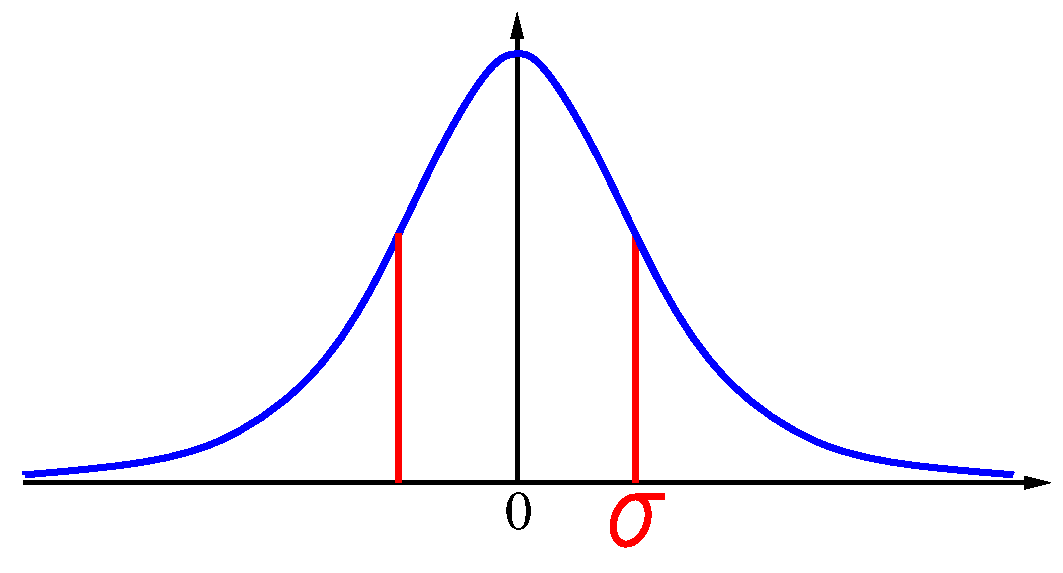
\includegraphics[height=1in]{gaussian-density}}
		\end{tabular}
	\end{block}
\end{frame}
\begin{frame}{Joint Probability Distributions}
	\begin{block}{Definition}
		\begin{tabular}{@{}lm{2.85in}@{}}
			\large $\mathbf{P}(X_1, \ldots, X_n)$
			&
			The \alert{joint probability distribution} of random variables $X_1, \ldots, X_n$ is a table of probabilities for each combination of values in the variable domains
		\end{tabular}
	\end{block}
	\pause
	\begin{block}{Example}
		$\mathbf{P}(\EM{Sex},\EM{Smoker}) = \mbox{}$ \\[.25em]
		\tab
		$
		\begin{array}{lcc}
			                           & \EM{Sex}\!=\!\EM{male} & \EM{Sex}\!=\!\EM{female} \\
			\EM{Smoker}\!=\!\EM{true}  & 0.113                  & 0.107 \\
			\EM{Smoker}\!=\!\EM{false} & 0.377                  & 0.403 \\
		\end{array}
		$
	\end{block}
\end{frame}
\begin{frame}{Full Joint Probability Distributions}
	\begin{block}{Definition}
		The \alert{full joint probability distribution} is the joint probability distribution for \emph{all variables that describe the world}
	\end{block}
	\pause
	\begin{block}{Example}
		$P(\EM{Sky},\EM{Temp}
		 \only<3->{,\EM{InBoulder}
		 \only<4->{,\EM{CarStolen}
		 \only<5->{,\EM{Cavity}
		 \only<6->{,\ldots}}}})$
	\end{block}
	\begin{block}<7>{More Seriously}
		\begin{itemize}
			\item We pick the variables we care about
			\item Full joint distribution uses those
		\end{itemize}
	\end{block}
\end{frame}


\subsection{Inference from Joint Distributions}
\begin{frame}{Inference with Joint Probability Distributions}
	\begin{block}{Key Idea}
		Sum entries in joint distribution where proposition is true
	\end{block}
	\pause
	\begin{block}{Example: $P(\EM{Sex}\!=\!\EM{female} \lor \EM{Smoker}\!=\!\EM{false})$}
		\tab\tab
		$
		\begin{array}{lcc}
			                           & \EM{Sex}\!=\!\EM{male} & \EM{Sex}\!=\!\EM{female} \\
			\EM{Smoker}\!=\!\EM{true}  & 0.113                  & 0.107 \\
			\EM{Smoker}\!=\!\EM{false} & 0.377                  & 0.403 \\
		\end{array}
		$
		\\ \medskip
		\pause
		$
		\begin{array}{lll}
			\lefteqn{P(\EM{Sex}\!=\!\EM{female} \lor \EM{Smoker}\!=\!\EM{false})} \\
			\pause
			& = & P(\EM{Sex}\!=\!\EM{male},\EM{Smoker}\!=\!\EM{false}) + \mbox{}\\
			&   & P(\EM{Sex}\!=\!\EM{female},\EM{Smoker}\!=\!\EM{true}) + \mbox{}\\
			&   & P(\EM{Sex}\!=\!\EM{female},\EM{Smoker}\!=\!\EM{false})\\
			\pause
			& = & 0.377 + 0.107 + 0.403 \pause = 0.887
		\end{array}
		$
	\end{block}
\end{frame}
\begin{frame}{Marginalization}
	\begin{block}{Key Idea}
		\begin{tabular}{lm{2.5in}}
			$
			\mathbf{P}(\mathbf{Y})
				= \sum\limits_{\mathbf{z}}{\mathbf{P}(\mathbf{Y}, \mathbf{z})}
			$
			&
			\alert{Marginalization} removes all variables but $\mathbf{Y}$ by summing over the values of the other variables
		\end{tabular}
	\end{block}
	\pause
	\begin{block}{Example: $P(\EM{Sex}\!=\!\EM{female})$}
		The other variable is $\EM{Smoker}$, so: \\[.5em]
		$
		\begin{array}{lll}
			\lefteqn{P(\EM{Sex}\!=\!\EM{female})} \\
			\pause & = & P(\EM{Sex}\!=\!\EM{female},\EM{Smoker}\!=\!\EM{true}) + \mbox{}\\
			       &   & P(\EM{Sex}\!=\!\EM{female},\EM{Smoker}\!=\!\EM{false})\\
			\pause & = & 0.107 + 0.403 \pause = 0.51
		\end{array}
		$
	\end{block}
\end{frame}
\begin{frame}{Inference Exercises}
	\begin{tabular}{@{}lm{2.2in}@{}}
		\small
		$
		\begin{array}{@{}l@{\hspace{.5em}}l@{\hspace{.5em}}l@{\hspace{.5em}}l@{}}
			\EM{sunny}  & \EM{warm} & \EM{snow}      & 0.01 \\
			\EM{sunny}  & \EM{warm} & \lnot\EM{snow} & 0.59 \\
			\EM{sunny}  & \EM{cold} & \EM{snow}      & 0.08 \\
			\EM{sunny}  & \EM{cold} & \lnot\EM{snow} & 0.14 \\
			\EM{cloudy} & \EM{warm} & \EM{snow}      & 0.03 \\
			\EM{cloudy} & \EM{warm} & \lnot\EM{snow} & 0.07 \\
			\EM{cloudy} & \EM{cold} & \EM{snow}      & 0.06 \\
			\EM{cloudy} & \EM{cold} & \lnot\EM{snow} & 0.02
		\end{array}
		$
		&
		\begin{enumerate}
			\item\small $P(\EM{sunny}) = \uncover<2>{0.82}$
			\item\small $P(\EM{warm}) = \uncover<2>{0.70}$
			\item\small $P(\EM{snow}) = \uncover<2>{0.18}$
			\item\small $P(\EM{sunny} \lor \lnot\EM{snow}) = \uncover<2>{0.91}$
			\item\small $P(\EM{sunny}|\EM{snow}) = \uncover<2>{0.50}$
			\item\small $P(\EM{snow}|\EM{sunny},\EM{cold}) = \uncover<2>{0.36}$
		\end{enumerate}
	\end{tabular}
\end{frame}
\begin{frame}{Full Joint Distribution Inference}
	\begin{block}{Properties}
		Given $n$ random variables with maximum domain size $d$: \\[1em]
		\begin{tabular}{ll}
			\key{Time Complexity?}  & \pause $O(d^{n})$ \\
			\pause
			\key{Space Complexity?} & \pause $O(d^{n})$
		\end{tabular}
	\end{block}
	\pause
	\begin{block}{Biggest Problem}
		How do you fill in a table of $O(d^{n})$ probabilities?
	\end{block}
\end{frame}

\section{Using Independence}
\subsection{Independence}
\begin{frame}{Independence}
	\begin{block}{Key Ideas}
		\begin{itemize}
			\item Sometimes no connection exists between variables
			\pause
			\item Such independence determined by world knowledge
		\end{itemize}
	\end{block}
	\pause
	\begin{block}{Formal Independence}
		$P(a, b) = P(a)P(b)$ \tab or \tab $P(a|b) = P(a)$
	\end{block}
	\pause
	\begin{block}{Examples}
		$
		\begin{array}{lll}
			\pause
			P(\EM{EyeColor},\EM{Gender}) & = & P(\EM{EyeColor})P(\EM{Gender}) \\
			\pause
			P(\EM{Cavity},\EM{BroncosWon}) & = & P(\EM{Cavity})P(\EM{BroncosWon}) \\
			\pause
			P(\EM{DieRoll}_{1},\EM{DieRoll}_{2}) & = & P(\EM{DieRoll}_{1})P(\EM{DieRoll}_{2}) \\
		\end{array}
		$
	\end{block}
\end{frame}
\begin{frame}{Independence}
	\begin{block}{Using Independence}
		\begin{itemize}
			\item No need to store entire joint probability table
			\item Can store several smaller independent tables
		\end{itemize}
	\end{block}
	\pause
	\begin{block}{Examples}
		$
		\begin{array}{ll}
		\mbox{\key{Distribution for}}              & \mbox{\key{Table Size}} \\
		\pause\mathbf{P}(\EM{DieRoll}_{1},
		                 \EM{DieRoll}_{2})         & \pause 6 \cdot 6 = 36 \\
		\pause\mathbf{P}(\EM{DieRoll}_{1})
		      \mathbf{P}(\EM{DieRoll}_{2})         & \pause 6 + 6 = 12 \\[.5em]
		\pause
		\mbox{\key{Distribution for}}              & \mbox{\key{Table Size}} \\
		\pause\mathbf{P}(\EM{Age}, \EM{Sex},
		                 \EM{BroncosWon})          & \pause 125 \cdot 2 \cdot 2 = 500 \\
		\pause\mathbf{P}(\EM{Age}, \EM{Sex})
		      \mathbf{P}(\EM{BroncosWon})          & \pause 125 \cdot 2 + 2 = 252 \\
		\end{array}
		$
	\end{block}
\end{frame}
\begin{frame}{Conditional Independence}
	\begin{block}{Key Idea}
		Two variables can sometimes become independent after the value of a third variable is observed
	\end{block}
	\begin{block}{Definition}
		A random variable $X$ is \alert{conditionally independent} of random variable $Y$ given the random variable $Z$ if: \\
		\tab$\mathbf{P}(X,Y|Z) = \mathbf{P}(X|Z)\mathbf{P}(Y|Z)$ \\
		or \\
		\tab$\mathbf{P}(X|Y,Z) = \mathbf{P}(X|Z)$
	\end{block}
\end{frame}
\begin{frame}{Conditional Independence Example}
	\begin{block}{Is $\EM{GrayHair}$ indpendent of $\EM{Bifocals}$?}
		\pause
		No, we expect the two to often come together, e.g.: \\[.5em]
		$P(\EM{gray-hair}, \EM{bifocals}) > P(\EM{gray-hair})P(\EM{bifocals})$
	\end{block}
	\pause
	\begin{block}{Is $\EM{GreyHair}$ independent of $\EM{Bifocals}$ given $\EM{Age}$?}
		\pause
		Yes, the bifocals add nothing if we know the age, e.g.: \\[.5em]
		$P(\EM{gray-hair}|\EM{bifocals},\EM{Age}=x) = P(\EM{gray-hair}|\EM{Age}=x)$
	\end{block}
\end{frame}
\begin{frame}{Conditional Independence Example}
	\begin{block}{Noisy Phone}
		\begin{itemize}
			\item Adam calls Betty and Charlie and says a number $N_{A}$
			\item Betty hears $N_{B}$ and Charlie hears $N_{C}$
		\end{itemize}
	\end{block}
	\pause
	\begin{block}{Are $N_{B}$ and $N_{C}$ independent?}
		\pause
		No, we expect the numbers to be similar, e.g.: \\[.5em]
		$P(N_{B}\!=\!1, N_{C}\!=\!1) > P(N_{B}\!=\!1)P(N_{C}\!=\!1)$
	\end{block}
	\pause
	\begin{block}{Are $N_{B}$ and $N_{C}$ conditionally independent given $N_{A}$?}
		\pause
		Yes, Betty's number adds nothing if we know Adam's, e.g.: \\[.5em]
		$P(N_{C}\!=\!1|N_{B}\!=\!2,N_{A}\!=\!1) = P(N_{C}\!=\!1|N_{A}\!=\!1)$
	\end{block}
\end{frame}


\subsection{Bayes' Rule}
\begin{frame}{Bayes' Rule}
	\begin{block}{Key Idea}
		Swap the conditioned and conditioning variables
	\end{block}
	\begin{block}{Bayes' Rule}
		\tab $\displaystyle P(b|a) = \frac{\displaystyle P(a|b)P(b)}{\displaystyle P(a)}$
	\end{block}
	\pause
	\begin{block}{Derivation}
		$
		\begin{array}{llll}
			P(b|a) & = & \pause\frac{\displaystyle P(a \land b)}
			                        {\displaystyle P(a)}         & \mbox{Definition} \\[1em]
			       & = & \pause\frac{\displaystyle P(a|b)P(b)}
			                        {\displaystyle P(a)}         & \mbox{Product Rule}
		\end{array}
		$
	\end{block}
\end{frame}
\begin{frame}{Why Use Bayes' Rule?}
	\begin{block}{Making Diagnoses Based on Causal Knowledge}
		$
		\displaystyle
		P(\EM{Cause}|\EM{Effect}) =
			\frac{\displaystyle P(\EM{Effect}|\EM{Cause})P(\EM{Cause})}
			     {\displaystyle P(\EM{Effect})}
		$
	\end{block}
	\pause
	\begin{block}{Example}
		\small
		$P(\EM{meningitis}|\EM{stiff{\scriptsize -}neck}) = 
			\frac{\displaystyle P(\EM{stiff{\scriptsize -}neck}|\EM{meningitis})
			                    P(\EM{meningitis})}
		       {\displaystyle P(\EM{stiff{\scriptsize -}neck})}
		$
		\\[1em]
		\pause
		In an epidemic, where $P(\EM{meningitis})$ rises: \\[.5em]
		\begin{tabular}{@{}l@{}l@{\hspace{.5em}}l@{}}
			\pause \key{+}&\key{Bayes}
			&
			\pause $P(\EM{meningitis}|\EM{stiff-neck})$ rises proportionally
			\\
			\pause \key{-}&\key{Bayes}
			&
			\pause Collect data, re-estimate $P(\EM{meningitis}|\EM{stiff-neck})$
		\end{tabular}
	\end{block}
\end{frame}
\begin{frame}{Bayes' Rule and Normalization}
	\begin{block}{Bayes' Rule}
		$\displaystyle P(b|a) = \frac{\displaystyle P(a|b)P(b)}
		                             {\displaystyle \alert<2->{P(a)}}$
		\tab\tab \uncover<3->{$P(b|a) = \alert{\alpha} P(a|b)P(b)$}
		\\[.5em]
		\uncover<2->{Treat $P(a)$ as a constant for normalizing to $[0, 1]$}
	\end{block}
	\begin{block}<4->{Calculating a Normalizing Constant}
		$
		\begin{array}{lllll}
		P(\mbox{A}|\spadesuit)P(\spadesuit)     & = & 1/13 \cdot 1/4 & =  & 1/52 \\
		P(\mbox{A}|\clubsuit)P(\clubsuit)       & = & 1/13 \cdot 1/4 & =  & 1/52 \\
		P(\mbox{A}|\diamondsuit)P(\diamondsuit) & = & 1/13 \cdot 1/4 & =  & 1/52 \\
		P(\mbox{A}|\heartsuit)P(\heartsuit)     & = & 1/13 \cdot 1/4 & =  & 1/52 \\[.5em]
		\uncover<5->{Total                      &   &                & =  & 1/13} \\
		\pause
		\uncover<6->{\alert{\alpha}             &   &                & =} & \uncover<7->{13} \\
		\end{array}
		$
	\end{block}
\end{frame}
\begin{frame}{Bayes' Rule and Conditional Independence}
	\begin{block}{Deriving More Manageable Models}
		$
		\begin{array}{lll}
		\lefteqn{P(\EM{Cavity}|\EM{toothache}, \EM{catch})} \\
		\pause
		& = & \alpha\displaystyle P(\EM{toothache}, \EM{catch}|\EM{Cavity})
		                          P(\EM{Cavity}) \\
		\pause
		& = & \alpha\displaystyle P(\EM{toothache}|\EM{Cavity})
		                          P(\EM{catch}|\EM{Cavity})
		                          P(\EM{Cavity}) \\
		\end{array}
		$
	\end{block}
	\pause
	\begin{block}{Naive Bayes Models}
		\small
		$
		P(\EM{Cause},\EM{Effect}_{1},\ldots,\EM{Effect}_{n})
		 = P(\EM{Cause})\prod_{i}{P(\EM{Effect}_{i}|\EM{Cause})}
		$
		\normalsize
		\begin{itemize}
			\item All effects conditionally independent given cause
			\item Common class of machine learning models
		\end{itemize}
	\end{block}
\end{frame}

\subsection{Wumpus World Example}
\begin{frame}{Wumpus World Example}
	\begin{columns}[T]
		\begin{column}{2.2in}
			\arrayrulewidth=2pt
			\begin{tabular}{@{}|@{}l@{}|@{}l@{}|@{}l@{}|@{}l@{}|@{}}
				\hline
				\wumpcell{1,4}{} &
				\wumpcell{2,4}{} &
				\wumpcell{3,4}{} &
				\wumpcell{4,4}{} \\
				\hline
				\wumpcell{1,3}{} &
				\wumpcell{2,3}{} &
				\wumpcell{3,3}{} &
				\wumpcell{4,3}{} \\
				\hline
				\wumpcell{1,2}{\uncover<2->{$\lnot P$ $B$}} &
				\wumpcell{2,2}{} &
				\wumpcell{3,2}{} &
				\wumpcell{4,2}{} \\
				\hline
				\wumpcell{1,1}{$\lnot P$} &
				\wumpcell{2,1}{\uncover<2->{$\lnot P$ $B$}} &
				\wumpcell{3,1}{} &
				\wumpcell{4,1}{} \\
				\hline
			\end{tabular}
		\end{column}
		\pause % for the uncovers above
		\begin{column}{2in}
			\pause
			\begin{block}{Query}
				$P_{1,3}$?
			\end{block}
			\pause
			\begin{block}{Brute Force Approach}
				\begin{itemize}
					\item Calculate full joint distribution
					\pause
					\item Sum the rows where:
					      $p_{1,3}$, $\lnot p_{1,1}$, $\lnot p_{1,2}$, $\lnot p_{2,1}$, $b_{1,2}$, $b_{2,1}$
					\pause
					\item Result is $P(p_{1,3})$
				\end{itemize}
			\end{block}
		\end{column}
	\end{columns}
\end{frame}
\begin{frame}{Wumpus World Brute Force}
	\begin{columns}[T]
		\begin{column}{2.2in}
			\arrayrulewidth=2pt
			\begin{tabular}{@{}|@{}l@{}|@{}l@{}|@{}l@{}|@{}l@{}|@{}}
				\hline
				\wumpcell{1,4}{} &
				\wumpcell{2,4}{} &
				\wumpcell{3,4}{} &
				\wumpcell{4,4}{} \\
				\hline
				\wumpcell{1,3}{} &
				\wumpcell{2,3}{} &
				\wumpcell{3,3}{} &
				\wumpcell{4,3}{} \\
				\hline
				\wumpcell{1,2}{} &
				\wumpcell{2,2}{} &
				\wumpcell{3,2}{} &
				\wumpcell{4,2}{} \\
				\hline
				\wumpcell{1,1}{} &
				\wumpcell{2,1}{} &
				\wumpcell{3,1}{} &
				\wumpcell{4,1}{} \\
				\hline
			\end{tabular}
		\end{column}
		\begin{column}{2.1in}
			\pause
			\begin{block}{Full Joint Distribution}
				\pause
				\small $\mathbf{P}(P_{11},\ldots,P_{44},B_{11},\ldots,B_{44})$
			\end{block}
			\pause
			\begin{block}{Total Rows?}
				\pause
				$2^{16 + 16} = 2^{32}$
			\end{block}
			\pause
			\begin{block}{Rows Selected?}
				Assume: \\
				\tab $p_{13}$ $\lnot p_{11}$ $\lnot p_{12}$ $\lnot p_{21}$ $b_{12}$ $b_{21}$
				\\[.5em]
				\pause
				$2^{12 + 14} = 2^{28}$
			\end{block}
			\pause
			There must be a better way!
		\end{column}
	\end{columns}
\end{frame}
\begin{frame}{Wumpus World with Independence}
	\begin{columns}[T]
		\begin{column}{2.2in}
			\arrayrulewidth=2pt
			\begin{tabular}{@{}|@{}l@{}|@{}l@{}|@{}l@{}|@{}l@{}|@{}}
				\hline
				\wumpcell{1,4}{\uncover<2->{\small Other}} &
				\wumpcell{2,4}{\uncover<2->{\small Other}} &
				\wumpcell{3,4}{\uncover<2->{\small Other}} &
				\wumpcell{4,4}{\uncover<2->{\small Other}} \\
				\hline
				\wumpcell{1,3}{\uncover<2->{\small \alert{Query}}} &
				\wumpcell{2,3}{\uncover<2->{\small Other}} &
				\wumpcell{3,3}{\uncover<2->{\small Other}} &
				\wumpcell{4,3}{\uncover<2->{\small Other}} \\
				\hline
				\wumpcell{1,2}{$\lnot P$ $B$} &
				\wumpcell{2,2}{\uncover<2->{\small \alert{Fringe}}} &
				\wumpcell{3,2}{\uncover<2->{\small Other}} &
				\wumpcell{4,2}{\uncover<2->{\small Other}} \\
				\hline
				\wumpcell{1,1}{$\lnot P$} &
				\wumpcell{2,1}{$\lnot P$ $B$} &
				\wumpcell{3,1}{\uncover<2->{\small \alert{Fringe}}} &
				\wumpcell{4,1}{\uncover<2->{\small Other}} \\
				\hline
			\end{tabular}
		\end{column}
		\begin{column}{2.2in}
			\begin{block}{Key Idea}
				Observations conditionally independent of other squares given neighboring squares
			\end{block}
			\begin{block}<4->{Goal}
				Manipulate equation until we can apply the conditional independence formula
			\end{block}
		\end{column}
	\end{columns}
	\medskip
	\uncover<3->{$\mathbf{P}(b_{12}, b_{21}|\lnot p_{11}, \lnot p_{12}, \lnot p_{21}, P_{13}, P_{\EMSCR{fringe}}, P_{\EMSCR{other}}) = \mathbf{P}(b_{12}, b_{21}|\lnot p_{11}, \lnot p_{12}, \lnot p_{21}, P_{13}, P_{\EMSCR{fringe}})$}
\end{frame}
\begin{frame}{Wumpus World Equation Manipulation}
	\begin{adjustwidth}{-1em}{-2em}
	\footnotesize
	$
	\begin{array}{lll}
	\lefteqn{P(p_{13}|\lnot p_{11}, \lnot p_{12}, \lnot p_{21}, b_{12}, b_{21})}
	\\
	\pause
	& = & \alpha
	      P(p_{13},
	        \lnot p_{11},
	        \lnot p_{12},
	        \lnot p_{21},
	        b_{12}, b_{21})
	\\
	\pause
	& = & \alpha
	      P(p_{13},
	        p_{\EM{\tiny known}},
	        b_{12}, b_{21})
	\\
	\pause
	& = & \alpha
	      \sum\limits_{\EM{\tiny fringe} + \EM{\tiny other}}
	      P(p_{13},
	        p_{\EM{\tiny known}},
	        p_{\EM{\tiny fringe} + \EM{\tiny other}},
	        b_{12}, b_{21})
	\\
	\pause
	& = & \alpha
	      \sum\limits_{\EM{\tiny fringe}}
	      \sum\limits_{\EM{\tiny other}}
	      P(p_{13},
	        p_{\EM{\tiny known}},
	        p_{\EM{\tiny fringe}},
	        p_{\EM{\tiny other}},
	        b_{12}, b_{21})
	\\
	\pause
	& = & \alpha
	      \sum\limits_{\EM{\tiny fringe}}
	      \sum\limits_{\EM{\tiny other}}
	      P(b_{12}, b_{21}|
	        p_{13},
	        p_{\EM{\tiny known}},
	        p_{\EM{\tiny fringe}},
	        p_{\EM{\tiny other}})
	      P(p_{13},
	        p_{\EM{\tiny known}},
	        p_{\EM{\tiny fringe}},
	        p_{\EM{\tiny other}})
	\\
	\pause
	& = & \alpha
	      \sum\limits_{\EM{\tiny fringe}}
	      \sum\limits_{\EM{\tiny other}}
	      P(b_{12}, b_{21}|
	        p_{13},
	        p_{\EM{\tiny known}},
	        p_{\EM{\tiny fringe}})
	      P(p_{13},
	        p_{\EM{\tiny known}},
	        p_{\EM{\tiny fringe}},
	        p_{\EM{\tiny other}})
	\\
	\pause
	& = & \alpha
	      \sum\limits_{\EM{\tiny fringe}}
	      \sum\limits_{\EM{\tiny other}}
	      P(b_{12}, b_{21}|
	        p_{13},
	        p_{\EM{\tiny known}},
	        p_{\EM{\tiny fringe}})
	      P(p_{13})
	      P(p_{\EM{\tiny known}})
	      P(p_{\EM{\tiny fringe}})
	      P(p_{\EM{\tiny other}})
	\\
	\pause
	& = & \alpha
	      \sum\limits_{\EM{\tiny fringe}}
	      P(b_{12}, b_{21}|
	        p_{13},
	        p_{\EM{\tiny known}},
	        p_{\EM{\tiny fringe}})
	      P(p_{13})
	      P(p_{\EM{\tiny known}})
	      P(p_{\EM{\tiny fringe}})
	      \sum\limits_{\EM{\tiny other}}
	      P(p_{\EM{\tiny other}})
	\\
	\pause
	& = & \alpha
	      \sum\limits_{\EM{\tiny fringe}}
	      P(b_{12}, b_{21}|
	        p_{13},
	        p_{\EM{\tiny known}},
	        p_{\EM{\tiny fringe}})
	      P(p_{13})
	      P(p_{\EM{\tiny known}})
	      P(p_{\EM{\tiny fringe}})
	\\
	\pause
	& = & \alpha
	      P(p_{13})
	      P(p_{\EM{\tiny known}})
	      \sum\limits_{\EM{\tiny fringe}}
	      P(b_{12}, b_{21}|
	        p_{13},
	        p_{\EM{\tiny known}},
	        p_{\EM{\tiny fringe}})
	      P(p_{\EM{\tiny fringe}})
	\end{array}
	$
	\end{adjustwidth}
\end{frame}
\begin{frame}{Wumpus World Probability Calculation}
	\begin{block}{Goal: Calculate the Summation}
		$
		\sum\limits_{p_{22}, p_{31}}
	  P(b_{12}, b_{21}|
	    p_{13},
	    \lnot p_{11},
	    \lnot p_{12},
	    \lnot p_{21},
	    P_{22},
	    P_{31})
	  P(P_{22},
	    P_{31})
		$
	\end{block}
	\pause
	\begin{block}{Key Ideas}
		\begin{itemize}
			\item First term is 1 if observed breezes are beside pits
			\item First term is 0 if observed breezes are not beside pits
			\pause
			\item So find worlds consistent with observations
			\item And sum $P(P_{22}, P_{31})$ over these worlds
		\end{itemize}
	\end{block}
\end{frame}
\begin{frame}{Wumpus World Probability Calculation}
	\begin{block}{Worlds Consistent with Observations}
		\begin{tabular}{@{}l@{\hspace{.2em}}l@{\hspace{.2em}}l@{\hspace{.2em}}l@{\hspace{.2em}}l@{}}
			\tinywumpusworld{\scriptsize\bf P}{$\lnot P$ $B$}{\scriptsize\bf P}{$\lnot P$}{$\lnot P$ $B$}{\scriptsize\bf P}
			&
			\tinywumpusworld{\scriptsize\bf P}{$\lnot P$ $B$}{\scriptsize\bf P}{$\lnot P$}{$\lnot P$ $B$}{}
			&
			\tinywumpusworld{\scriptsize\bf P}{$\lnot P$ $B$}{}{$\lnot P$}{$\lnot P$ $B$}{\scriptsize\bf P}
			&
			\tinywumpusworld{}{$\lnot P$ $B$}{\scriptsize\bf P}{$\lnot P$}{$\lnot P$ $B$}{\scriptsize\bf P}
			&
			\tinywumpusworld{}{$\lnot P$ $B$}{\scriptsize\bf P}{$\lnot P$}{$\lnot P$ $B$}{}
			\\
			\uncover<3->{\scriptsize $0.2\!\times\!0.2\!=\!0.04$}
			&
			\uncover<4->{\scriptsize $0.2\!\times\!0.8\!=\!0.16$}
			&
			\uncover<5->{\scriptsize $0.8\!\times\!0.2\!=\!0.16$}
			&
			\uncover<6->{\scriptsize $0.2\!\times\!0.2\!=\!0.04$}
			&
			\uncover<7->{\scriptsize $0.2\!\times\!0.8\!=\!0.16$}
			\\
			\uncover<2->{\lefteqn{\mbox{Calculating $P(P_{22}, P_{31})$, assuming pit probability is 0.2}}} \\
		\end{tabular}
	\end{block}
	\begin{block}<8->{Final Calculation}
		\begin{itemize}
			\item $\sum\limits_{p_{22}, p_{31}}P(b_{12}, b_{21}|p_{13},\ldots)P(P_{22},P_{31}) = 0.04 + 0.16 + 0.16$
			\item $\sum\limits_{p_{22}, p_{31}}P(b_{12}, b_{21}|\lnot p_{13},\ldots)P(P_{22},P_{31}) = 0.04 + 0.16$
		\end{itemize}
	\end{block}
\end{frame}
\begin{frame}{Wumpus World Probability Calculation}
	$
	\begin{array}{lll}
	\lefteqn{P(p_{13}|\lnot p_{11}, \lnot p_{12}, \lnot p_{21}, b_{12}, b_{21})}
	\\
	\pause
	& = &
	\alpha
	P(p_{13})
	P(\lnot p_{11},\lnot p_{12},\lnot p_{21})
	\sum\ldots p_{13}\ldots
	\\
	\pause
	& = &
	\alpha \!\times\!
  0.2 \!\times\!
	P(\lnot p_{11},\lnot p_{12},\lnot p_{21})
	\sum\ldots p_{13}\ldots
  \\
  \pause
  & = &
  \alpha \!\times\!
  0.2 \!\times\!
  0.8 \!\times\! 0.8 \!\times\! 0.8 \!\times\!
  \sum\ldots p_{13}\ldots
  \\
  \pause
  & = &
  \alpha \!\times\!
  0.2 \!\times\!
  0.8 \!\times\! 0.8 \!\times\! 0.8 \!\times\!
  (0.04 + 0.16 + 0.16)
  \\
  \pause
  & = & 0.036864\alpha
  \\[1em]
  \pause
	\lefteqn{P(\lnot p_{13}|\lnot p_{11}, \lnot p_{12}, \lnot p_{21}, b_{12}, b_{21})}
	\\
	\pause
	& = & 
	\alpha
	P(\lnot p_{13})
	P(\lnot p_{11},\lnot p_{12},\lnot p_{21})
	\sum\ldots \lnot p_{13}\ldots
  \\
  \pause
  & = &
  \alpha \!\times\!
  0.8 \!\times\!
  0.8 \!\times\! 0.8 \!\times\! 0.8 \!\times\!
  (0.04 + 0.16)
  \\
  \pause
  & = & 0.08192\alpha
  \\[1em]
  \pause
  \lefteqn{P(p_{13}|\lnot p_{11}, \lnot p_{12}, \lnot p_{21}, b_{12}, b_{21})}
  \\
  \pause
  & = & 0.036864 / (0.036864 + 0.08192) \approx 0.31
  \end{array}
  $
\end{frame}

\part{Key Ideas}
\begin{frame}{Probability Rules}
	\begin{columns}
		\begin{column}{2in}
			\begin{block}{Product Rule}
				$P(a,b) = P(a|b)P(b)$
			\end{block}
			\begin{block}{Independence}
				$P(a,b) = P(a)P(b)$
			\end{block}
			\begin{block}{Conditional Independence}
				$P(a,b|c) = P(a|c)P(b|c)$ \\
				$P(a|b,c) = P(a|c)$ \\
			\end{block}
		\end{column}
		\pause
		\begin{column}{2.4in}
			\small
			Given: 
			\begin{tabular}[t]{l}
				$a$ indep. $b,c,d$ \\
				$b$ indep. $d$ given $c$
			\end{tabular}
			\\ \smallskip
			Show:
			\\ \smallskip
			$
			\begin{array}{l}
				P(a,b,c,d) = P(a)P(b|c)P(d,c)
			\end{array}
			$
			\\ \bigskip
			\pause
			Proof:
			\\ \smallskip
			$
			\begin{array}{@{}ll@{}}
			\lefteqn{P(a,b,c,d)} \\
			\pause = P(a)P(b,c,d)         & \pause\mbox{Indep.} \\
			\pause = P(a)P(b,d|c)P(c)     & \pause\mbox{Product} \\
			\pause = P(a)P(b|c)P(d|c)P(c) & \pause\mbox{Cond.} \\
			\pause = P(a)P(b|c)P(d,c)     & \pause\mbox{Product} \\
			\end{array}
			$
		\end{column}
	\end{columns}
\end{frame}
\begin{frame}{Probability Rule Exercises}
	\begin{columns}
		\begin{column}{2in}
			\begin{block}{Product Rule}
				$P(a,b) = P(a|b)P(b)$
			\end{block}
			\begin{block}{Independence}
				$P(a,b) = P(a)P(b)$
			\end{block}
			\begin{block}{Conditional Independence}
				$P(a,b|c) = P(a|c)P(b|c)$ \\
				$P(a|b,c) = P(a|c)$ \\
			\end{block}
		\end{column}
		\begin{column}{2.4in}
			\small
			Given: \\
			\begin{tabular}[t]{l}
				$d$ indep. $a,b,c$ \\
				$a$ indep. $b$ given $c$
			\end{tabular}
			\\ \smallskip
			Show:
			\\ \smallskip
			$
			\begin{array}{l@{}}
				P(a,d|b,c) = P(a|c)P(d)
			\end{array}
			$
			\\ \bigskip
			Given: \\
			\begin{tabular}[t]{l}
				$a$ indep. $c,d$ given $b$ \\
				$b$ indep. $d$ given $c$ \\
				$c$ indep. $d$
			\end{tabular}
			\\ \smallskip
			Show:
			\\ \smallskip
			\footnotesize
			$
			\begin{array}{l@{}}
				P(a,b,c,d) = P(a|b)P(b|c)P(c)P(d)
			\end{array}
			$
		\end{column}
	\end{columns}
\end{frame}
\begin{frame}{Normalization Rules}
	\begin{columns}
		\begin{column}{2in}
			\begin{block}{Complements}
				$P(\lnot a) + P(a) = 1$
			\end{block}
			\begin{block}{Summing Out}
				$P(a, b) + P(\lnot a, b) = P(b)$
			\end{block}
			\begin{block}{Distributions}
				$\sum\limits^{d}_{i}{P(X=x_{i})} = 1$
			\end{block}
		\end{column}
		\pause
		\begin{column}{2.4in}
			\small
			Given: $\mathbf{P}(A|b,c) = \alpha\langle 0.1, 0.3 \rangle$
			\\ \smallskip
			Show: $\mathbf{P}(A|b,c) = \langle 0.25, 0.75 \rangle$
			\\ \bigskip
			\pause
			$
			\begin{array}{@{}l@{\hspace{.2em}}l@{\hspace{.2em}}l@{}}
			P(b,c) & = & P(a,b,c) + P(\lnot a,b,c) \\[.2em]
			\pause
			1      & = & \displaystyle\frac{P(a,b,c) + P(\lnot a,b,c)}{P(b, c)} \\[.8em]
			\pause
			1      & = & \displaystyle\frac{P(a,b,c)}{P(b, c)} + \frac{P(\lnot a,b,c)}{P(b, c)} \\[.8em]
			\pause
			1      & = & \displaystyle\frac{P(a,b,c)}{P(b, c)} + \frac{P(\lnot a,b,c)}{P(b, c)} \\[.8em]
			\pause
			\alert<11->{1} & = & \alert<11->{P(a|b,c) + P(\lnot a|b,c)} \\[.2em]
			\pause
			1      & = & 0.1\alpha + 0.3\alpha \\[.2em]
			\pause
			1      & = & 0.4\alpha \\[.2em]
			\pause
			2.5    & = & \alpha
			\end{array}
			$
		\end{column}
	\end{columns}
\end{frame}
\begin{frame}{Normalization Rule Practice}
	\begin{columns}
		\begin{column}{2in}
			\begin{block}{Complements}
				$P(\lnot a) + P(a) = 1$ \\
				$P(a|b) + P(\lnot a|b) = 1$
			\end{block}
			\begin{block}{Summing Out}
				$P(a, b) + P(\lnot a, b) = P(b)$
			\end{block}
			\begin{block}{Distributions}
				$\sum\limits^{d}_{i}{P(X=x_{i})} = 1$
			\end{block}
		\end{column}
		\begin{column}{2.4in}
			\small
			Given:
			\\ \smallskip
			$
			\begin{array}{lll}
				P(b|a)       & = & 0.4 \\
				P(b|\lnot a) & = & 0.9 \\
				P(a)         & = & 0.2 \\
				P(\lnot a)   & = & 0.8
			\end{array}
			$
			\\ \bigskip
			Show: $\mathbf{P}(A|b) = \langle 0.1, 0.9 \rangle$
		\end{column}
	\end{columns}
\end{frame}
\begin{frame}{Key Ideas}
	\begin{block}{Probability Measures Belief}
		$P(\EM{false}) = 0$ \tab $P(\EM{true}) = 1$ \tab\tab\tab $\sum\limits_{x}P(X\!=\!x) = 1$
	\end{block}
	\begin{block}{Types of probabilities}
		\begin{itemize}
			\item Prior, $P(X\!=\!x)$
			\item Joint, $P(X\!=\!x,Y\!=\!y)$
			\item Conditional, $P(X\!=\!x|Y\!=\!y)$
		\end{itemize}
	\end{block}
	\begin{block}{Inference}
		\begin{itemize}
			\item Sums over full joint distribution
			\item Conditional independence + product and Bayes' rule
		\end{itemize}
	\end{block}
\end{frame}

\end{document}


